\documentclass[uplatex,a4j]{jsreport}
\usepackage{thesis}

\begin{document}
\chapter{序論}

自然言語は、人間が同士が互いにコミュニケーションをとるために発展してきた言語である.そして自然言語をコンピュータにで処理する技術を自然言語処理(Natural Language Processing)と呼んでいる.
本論文では自然言語処理の技術を使ってHTML5の字句解析仕様から命令を抽出することを試みた.

図\ref{流れ}がHTML5の字句解析仕様の意味解析の概要である.\\
% 概要の図
\begin{figure}[h]
    \centering
    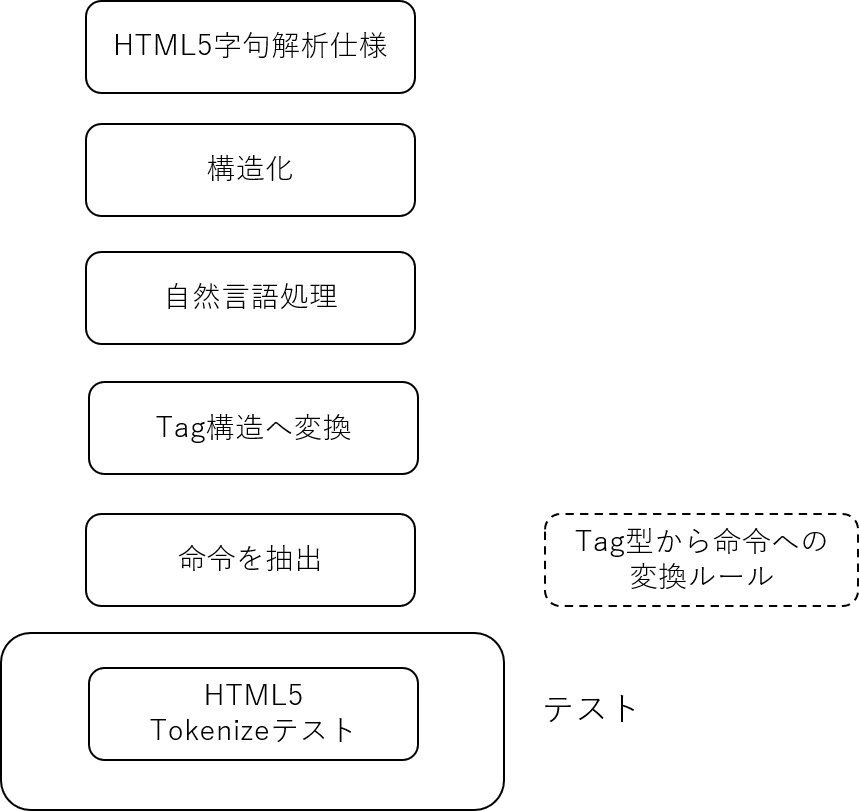
\includegraphics[keepaspectratio, scale=0.6]
         {figure/流れ.png}
    \caption{流れ(仮)}
    \label{流れ}
\end{figure}
\\
% ここの部分を何章で説明する、とかを書く
本論文では, まず\ref{準備}章で自然言語処理の基礎知識を述べる.
次に\ref{字句解析仕様}章で HTML5 の字句解析器の主な仕様, 動作について述べる.
\ref{形式}章で抽出する命令の形式をBNFとして述べ, 
\ref{自然言語処理}章で自然言語処理ライブラリを用い, それをHTML5字句解析仕様に適用させ, 
\ref{命令抽出}章で自然言語処理の出力をもとに仕様書の命令の抽出を行った. 
\ref{実装}章で抽出した命令をもとに字句解析をするインタプリターを作成し, 
\ref{評価}章で字句解析のテストデータを用い, 抽出した命令の正しさを検証した.
\end{document}